\section{API Django Rest Framework}
Esta sessão tratará sobre o servidor do sistema, também conhecido como \textit{backend}
ou API Django. Na primeira subsessão, é tratada uma breve descrição sobre as funções
e características deste. A segunda apresenta o \textit{design} e a arquitetura
de desenvolvimento. Por fim, trataremos as instâncias do projeto desenvolvido.


\subsection{Papel da API}
\label{sub:papel_da_api}
O backend do sistema, responsável por fazer o controle das requisições,
atuando como intermediador à cadeira e aos seus respectivos monitores   
foi desenvolvida utilizando o \textit{Django Rest Framework}. Este é uma
referência no mundo de desenvolvimento \textit{Python} para \textit{API's Rest}.

O backend manipula todos os dados enviados pela cadeira, utilizando a \textit{Rasp}
executa o processamento destes dados e envia notificações para os \textit{Smartphones}
cadastrados no sistama. Além disso, serve dados para uma interface web de controle
do monitor.

A manipulação dos dados é feita de forma segura, tratando a autenticação dos usuários
que lidam com o sistema e redirecionando os dados de acordo com a sua autenticação.
Para executar estes passos, o servidor conta com um poderoso sistema de autencação
dos seus usuários, tanto para os pacientes que utilizam a cadeira, quanto para os
monitores que manipulam as interfaces para cliente, como mobile e interface web.
Os pacientes são cadastrados no sistema e enviam os sinais corporias para o servidor.
O servidor, além de enviar uma notificação para o monitor respectivo, armazena este
sinal em sua base de dados e retorna ao monitor quando solicitado.
Os dados enviados ao monitor são apenas os sinais respectivos ao paciente que está
sendo monitorado.

A ligação entre o paciente e o monitor pode ser feita no momento do cadastro ou em
atualizações futuras. O paciente contém um identificador único em sua cadeira, que
pode ser utilizada pelo monitor para supervisioná-lo. No momento que o monitor insere
os dados no sistema, automaticamente serão ligados e o monitor terá acesso aos dados
de sinais enviados pelo paciente.

\subsection{\textit{Design} e Arquitetura da Solucação}
\label{sub:design_e_arquitetura_da_soluca_o}

O django utiliza de uma arquitetura própria para padronização e aplicação de boas
práticas em desenvolvimento de API's. Esta arquitetura está dividida em camadas,
que são responsáveis por funções específicas e cada uma tem seu papel definido
para a manipulação de dados no sistema. A seguir está uma ilustração do funcionamento
da arquitetura do servidor. 

\begin{figure}
    \begin{center}
        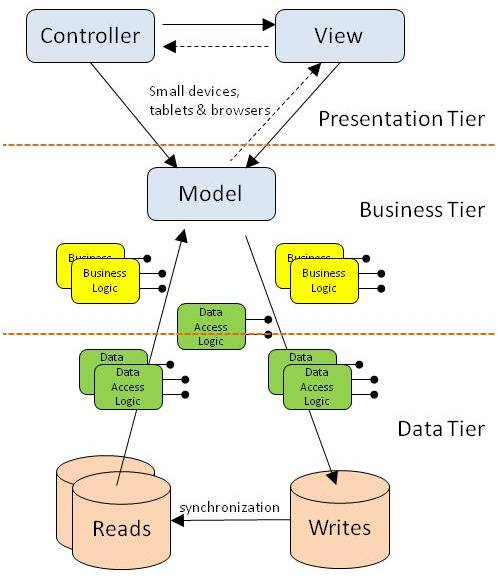
\includegraphics[scale=1]{figuras/rest_arch.jpg}
    \end{center}
    \caption{\textit{Design} e Arquitetura do servidor Django}
    \label{fig:rest_arch}
\end{figure}

Como pode ser observado, existem três camadas principais, que são utilizadas
para a manipulação dos dados. Elas são:

\begin{itemize}
    \item Presentation Tier;
    \item Business Tier;
    \item Data Tier.
\end{itemize}

A primeira, \textit{Presentation Tier} é resposável por ser a interface com as demais aplicações
que irão utilizar os servidor. Essa camada é responsável por gerir as rotas do sistema, direcionando
as urls solicitadas a funções específicas. Após mapeado nas funções, estas irão verificar as permissões
de cada requisição, bem como cada usuário que está solicitando uma determinada ação.

As funções mapeadas na Tier passada utiliza de modelos preedefinidas na Tier de Business.
Aqui são definidos os domínios da aplicação, bem como quais são as classes e negócio da
aplicação. Nesta fase são definidos os tipos de usuários do sistema, as classes de sinais
corporais do paciente e toda parte a de negócios da aplicação.

A última camada, chamada de \textit{Data Tier} é responsável por lidar com a persistência dos dados
de todos os usuários e sinais que são manipulados no sistema. Esta camada modela o
bando de dados assim como foi definido na aplicação de negócios e aplica
inserções neste a medida que novas requisições são feitas.
